\chapter{移动用户行为分析平台}
\label{cha:system}

\section{系统概述}
\label{system:sec:intro}
移动环境下的用户行为数据,具有数据量巨大,数据种类繁多,来源多种多样等特点。如何将大量的异构数据进行有效的整合和高校的处理、挖掘,是在移动环境下进行用户行为分析所面临的重要挑战。本章描述的\textbf{移动用户行为分析平台(Mobile Data Analysis Platform,MDAP)},是一个集数据收集、存储、计算和展示为一体的全面的云计算数据挖掘平台。

本平台可分为底层数据存储、统一化的数据集操控API、REST API、可制定数据挖掘模块、数据展示和可视化模块等部分组成。平台的组织架构参见图\ref{mdap:fig:architecture}。

\begin{figure}[htbp]
  \centering
    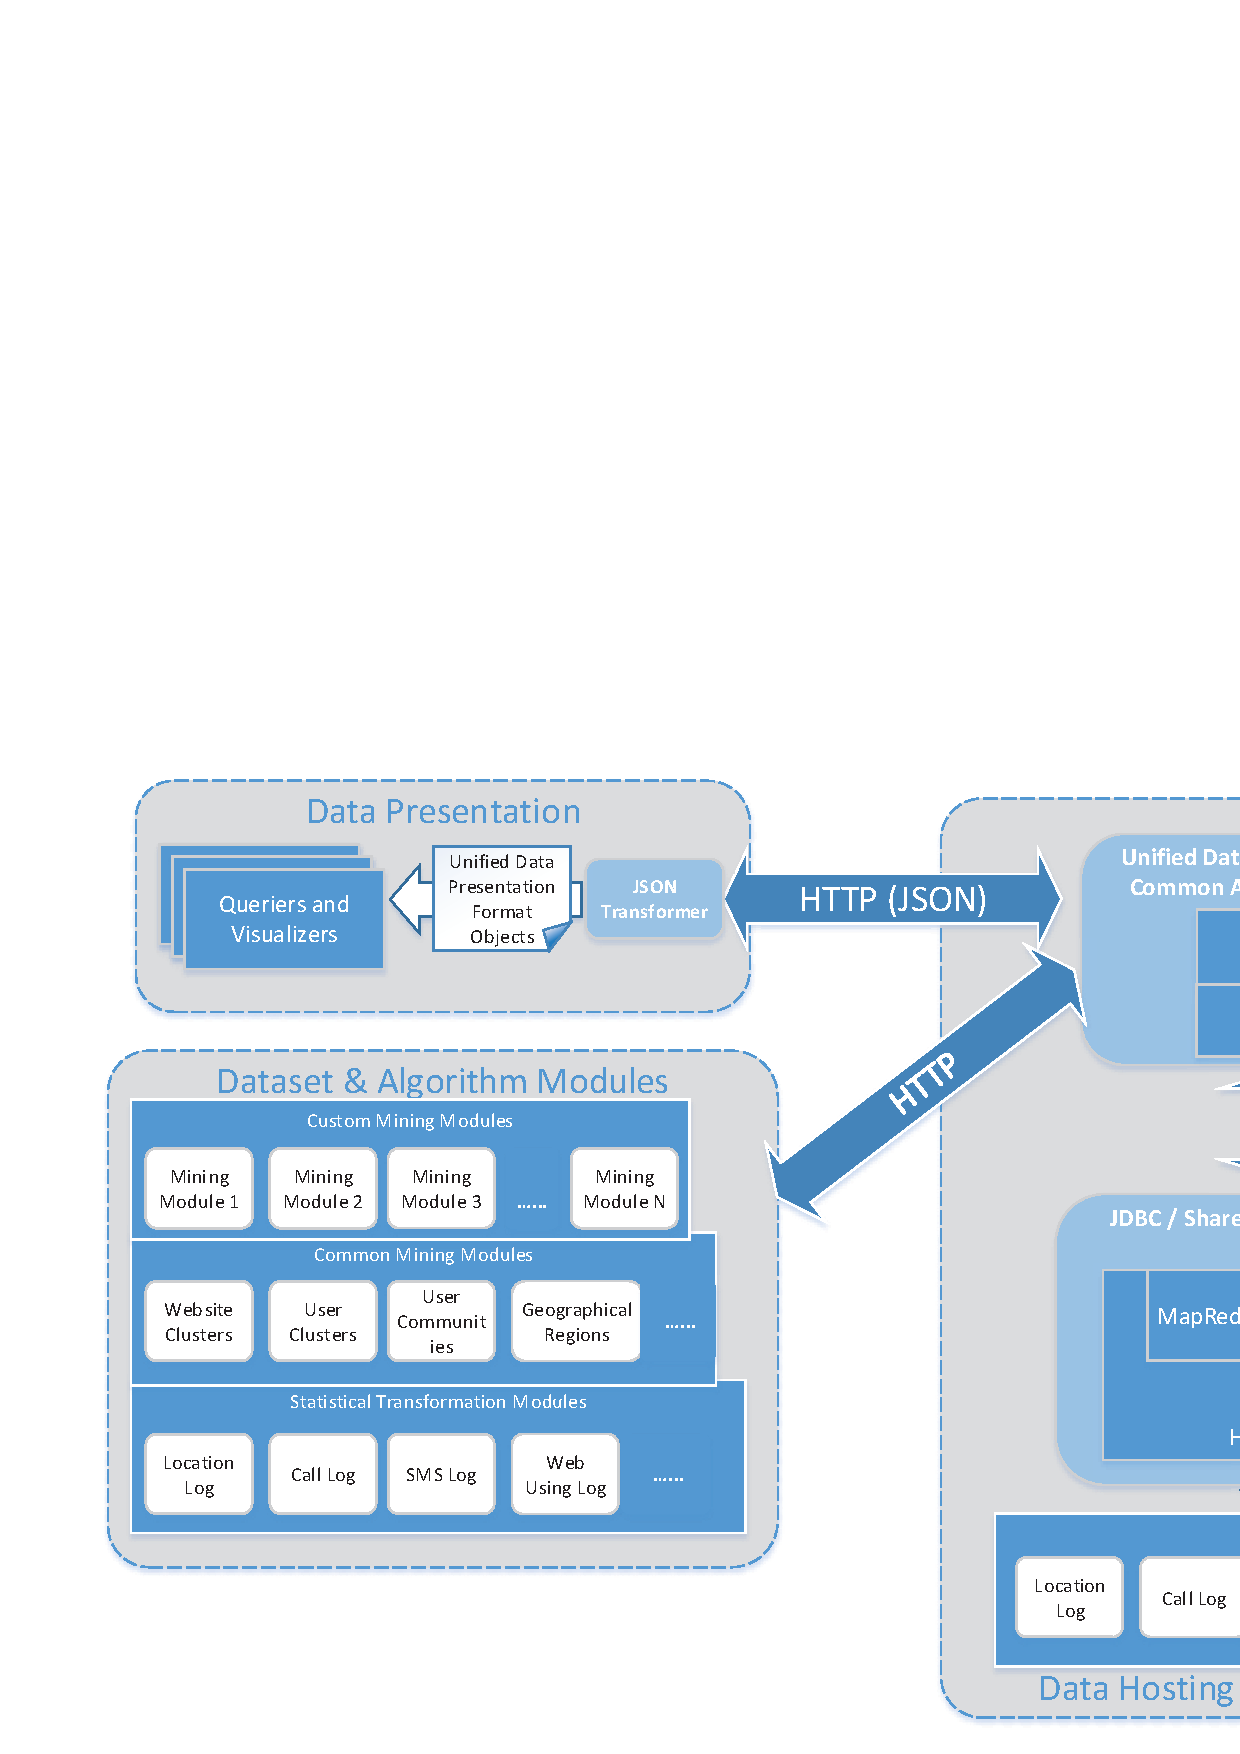
\includegraphics[width=15cm]{mdap}
  \caption{MDAP组织架构图}
  \label{mdap:fig:architecture}
\end{figure}

平台主要提供表格式数据集的添加、访问、增加和删除。在数据的来源方面,平台支持流式的数据输入,可以从移动运营商处通过文件复制或访问数据接口等方式导入,也可由手机客户端通过访问API来写入。平台的手机客户端应用,可以使用不同策略采集多种手机传感器的数据,以及通讯数据和其他手机使用数据。关于手机端采集系统的实现详见第\ref{system:sec:collect}章。

在数据的存储方面,平台底层支持多种异构的数据存储方式,包括Hadoop/HDFS,Hive,SQL关系数据库,以及文本文件等等。数据的存储的运算是否为并行化取决于其低层的的数据存储实现方式。不同的数据存储实现方式通过统一的编程API提供数据操控服务,从而屏蔽了底层实现的异构性,使平台的使用者(数据挖掘研究人员和数据分析师)能够不必关系底层数据存储实现方式,而专注于数据和对数据的分析挖掘。

数据的访问方面,对于挖掘中使用率最高的表格型数据,平台规定了一整套抽象的统一接口,包括数据集元数据的表示方式,数据的查询接口、返回格式和遍历方法,以及数据的写入方法等。关于编程接口的详细描述参见第\ref{system:sec:javaapi}章。同时,平台还提供标准的REST API,给开发者和可视化人员提供远程调用的接口。关于REST接口的详细描述见第\ref{system:sec:restapi}章。

在数据展示方面,不同类型的数据集携带了不同的语义信息(如地理位置、时间序列数据、统计数据等),根据数据集的语义信息可以知道其适合使用哪种形式的图表予以可视化。平台的数据可视化模块,可以根据数据集语义信息API中获取的语义信息对数据集进行通用而又有针对性的可视化展示。有关可视化系统详见第\ref{system:sec:vis}章。



\section{手机端数据采集系统}
\label{system:sec:collect}

手机端产生的传感器数据、通讯数据及手机使用数据等,对用户个体的行为分析十分重要。手机端的数据采集采用手机应用的方式,采集多种不同的手机产生的数据,经过简单的处理转换,而后自动上传到平台中供集中存储和分析。

目前的手机端数据采集应用运行于Android平台。由于手机上的传感器类型及其他类型数据在不同平台上都类似,所以此应用也可以很简单地扩展到其他平台。

\subsection{Android平台传感器概述}
\label{system:sec:AndroidPlatformSensors}

\textbf{Android} \footnote{\url{http://www.android.com/}} 是一个应用于移动设备(手机,平板电脑等)等基于Linux的操作系统\footnote{\url{http://en.wikipedia.org/wiki/Android_(operating_system)}}。
Android包含一个基于Linux的定制内核,以及一个针对移动环境优化过的虚拟运行时环境,称为Dalvik。Android上运行的应用通常由Java语言编写,而后便以为Dalvik的dex-code,而后运行于Dalvik平台。从2007年项目开始至今,Android已经成长为世界上使用最为广泛的智能手机操作系统。 

Android内置支持多种传感器设备。目前,版本号16的Android API描述了11种传感器类型\footnote{\url{http://developer.android.com/reference/android/hardware/Sensor.html}},新的传感器类型还在不断加入中。Android设备方面,声音传感器(麦克风),位置感知功能(通过GPS、WIFI等)以及加速度传感器已几乎成为Android手机的标配。然而,由于采用Android系统的设备种类繁多,并不能保证某一种类的传感器一定会存在于某一台设备上。本系统中采集的传感器数据类型同时考虑了其在不同设备上的可用性以及对用户行为建模的作用。

Android使用广播-接受模式(broadcaster-receiver pattern)来管理传感器。当某一应用需要使用传感器时,首先要向系统注册为该传感器的接收者,与此同时,指定一个接收传感器数据的敏感程度(用以控制频率)。而后,每当传感器的感知数值发生变化(由所设置的敏感程度控制)\cite{sensorevent}。

\begin{itemize}
  \item \textbf{加速度传感器.} Android系统的加速度传感器数据的计算是通过测量传感器本身的受力实现的,其中也包含重力。根据Android系统的三轴定位系统,加速度传感器的读书包含三部分:X轴位水平向右方向,Y轴为垂直向上,Z轴垂直于屏幕向外\cite{sensorevent}。将$t$时刻的的加速度传感器数值即为$(x^{(t)}, y^{(t)}, z^{(t)})$。
  
  加速度传感器可能是Android设备商配备率最高的传感器,而且其能量消耗也较低。加速度传感器数据可以用于探测用户的物理移动情况,这在行为建模上十分重要。
  基于以上原因,加速度传感器在所有传感器数据中处于核心地位。

  \item \textbf{声音传感器.} 严格来说,声音传感器并不属于Android系统的传感器类型。然而,每一部手机都配备有麦克风,可以用来感知用户的声音以及背景声音的强弱。在心境建模方面,环境声音的状态能用影响到用户的心境状态,而用户的声音也能够反映到其心境状态。
  \item \textbf{地理位置.} 地理位置和用户行为也有着紧密的联系,可以作为用户行为的一个重要的上下文信息。Android提供了两种地理位置信息:粗略位置服务和精确位置服务。地理位置可以通过GPS,WiFi以及移动蜂窝网络来获得。由GPS提供的精确位置能够达到3米以内的精度;不使用GPS的定位能够达到数十米的精度,但对于用户行为建模的楼宇级别的定位,这一精度也在可以接受的范围之内。
  \item \textbf{光线传感器.} 环境光线传感器一般用来自动调整屏幕的亮度,控制键盘背景灯等等能。背景光线情况能够反映用户所处的环境,影响到用户的行为。同时,环境光线还能够用来判定手机所处的位置(在衣服口袋里,桌上等)。
\end{itemize}

\subsection{应用实现}
\label{system:sec:ApplicationImplementation}

收集数据手机应用包含如下的数据收集组件:传感器数据收集;通讯数据收集;其他信息收集(如用户情绪自报告)。 

应用的工作流程如下。传感器数据的收集随着应用的启动而开始。对不同类型的传感器数据采用不同的策略记录下来(后文详细描述),收集的传感器数据暂时以文本文件的形式存储于手机内。(Android系统内置有SQLite数据库支持,但其在大量数据的顺序读写上的效率远低于使用纯文本文件,故此处未予采用)。
%
通讯数据的收集发生在每次数据上传行为前,从Android系统的系统日志中获得。通讯信息获取模块从手机中读取短信和通话记录信息,将其中的目标号码,时间以及长度信息存储于手机文本文件中。这些数据可以用来作为通讯频率统计数据来源,也可以作为建立社交网络的数据源。
%
其他信息收集为面向某一特定挖掘任务所需要收集的特殊类型的信息,如心境评估问题中需要的用户心境自报告。心境自报告模块包含一个允许用户报告其心境的图形界面。应用的使用者每天至少一次,每次以三个维度(每个维度有5个离散级别)报告其心境状态。根据应用的设置,每晚十点钟用户情绪报告页面会自动弹出,但用户也可在任何时间通过菜单调出报告界面。此类其他信息同样被以文本文件的形式存储与手机中。

每天手机的数据会在当日末尾上传到平台上。首先在本地将存有传感器数据,通讯数据以及其他数据的文本文件进行压缩,而后在手机有可用的数据连接(移动网络或WiFi,用户可设置)的时候自动上传。

除了基本的数据格式转换外,所有的原始数据都被上传到云端,其余的处理和挖掘工作全部在云端完成。用户可以通过应用获取平台提供的挖掘结果,应用也可以调用平台的数据可视化接口向用户展示统计和挖掘的结果。

图\ref{system:fig:interface}展示了用于心境评估中的应用界面截图。该界面中显示了计算得到的用户行为特征。界面底部给出的心境的评估结果。

\begin{figure}[htbp]
  \centering
    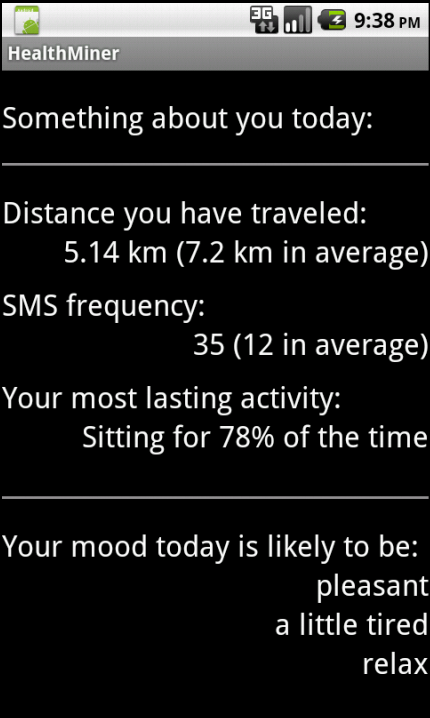
\includegraphics[width=215bp,natwidth=430bp,natheight=718bp]{interface.png}
  \caption{手机端数据展示界面(包括心境)}
  \label{system:fig:interface}
\end{figure}

\subsection{传感器管理策略}
\label{system:sec:SensorManagementStrategy}

手机传感器通常有较高的能耗,高强度地使用手机传感器将会显著地影响手机的电池寿命。在本应用中,针对不同的传感器,使用了不同的生命周期管理方法,从而达到了适应数据采集需要和降低能耗之间的平衡。

对能耗影响最大的两个传感器类型是加速度传感器和定位传感器。

加速度传感器在Android手机上配备最为广泛,其能耗功率也比较低,我们在平台中将加速度传感器数据作为一直需要采集的数据,用来进行用户的姿态检测,动作检测等(示例详见第\ref{mood:sec:ProblemAndFeatureDefinition}章)。然而,虽然加速度传感器的功率相对较低,但由于其数据需求的频率比较高,因此对加速度传感器的管理对最终能耗有较大影响。
% 
当应用接收到加速度传感器数据时,首先将其和之前的读数进行比较。如果新值与原值间的差别不大,认为手机状态没有发生显著变化,则新值不会保存,而且会适当降低数据采样的频率。只有两个值之间差别较大时,说明手机的物理运动状态发生了显著改变(如:被用户用手拿起),才会记录新的加速度值。基于实验观察,最终确定,只有三个轴上的任何一个的读书变化0.5m/s$^2$时才视为显著变化。
  
另一个高耗能的传感数据类型为地理位置。地理位置通常通过GPS或WiFi等渠道获得,这两种方式能耗都比较大。参考Cui等\cite{jianc}的做法,本应用将加速度传感器数据和地理位置相结合,设计了一个自适应的地理位置感知方法。
具体地,在预先设置的时间片$T$内,用加速度传感器的读数粗略地估算地理位置的变化。如果算出的地理位置变化并不明显,意味着设备处于一个相对稳定的状态,这时并不激活GPS或WiFi等位置传感器,而是将上次测得的位置作为当前的位置。为消除累积误差,同时要保证位置传感器在每$T_0$时间段内至少要启动一次。这个策略能够较为精确地感知地理位置,同时显著降低了传感器能耗。


\section{并行化数据分析平台}
\label{system:sec:mdap}
\subsection{平台编程接口的设计与实现}
\label{system:sec:javaapi}
在平台中,所有对底层数据的操作被一套抽象的API所封装,对数据的一切操作都需要通过API调用来实现。API采用Java编程语言,包含了数据集元数据管理,数据查询和访问,数据操纵,数据集语义信息管理等功能。整套API框架中的顶层接口规范见图\ref{system:fig:javaapi}

\begin{figure}[htbp]
  \centering
    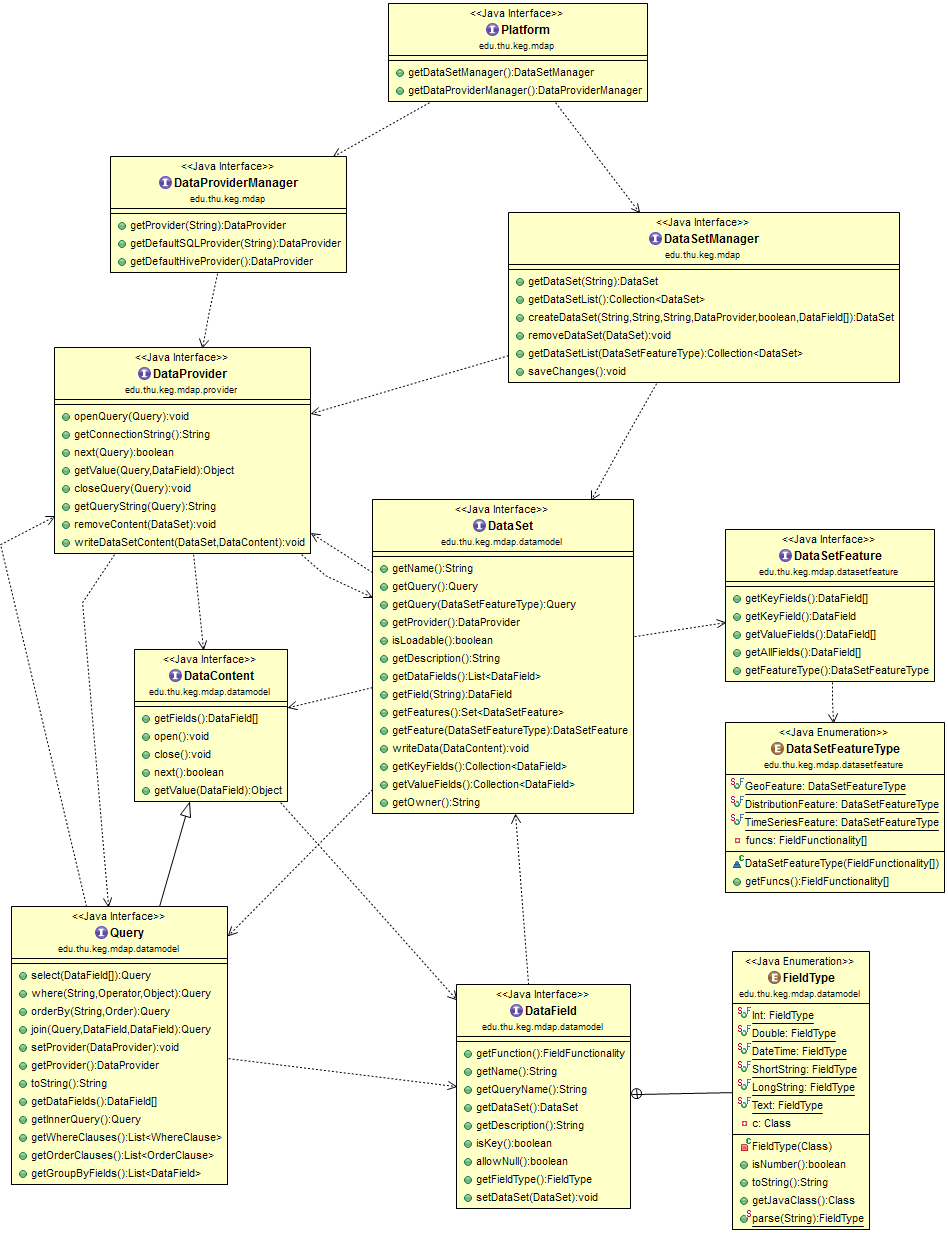
\includegraphics[width=15cm]{api.png}
  \caption{MDAP顶层编程接口规范}
  \label{system:fig:javaapi}
\end{figure}

\textbf{数据集元数据管理.} 
\textbf{数据集}是本平台中管理数据的基本概念。每个数据集描述了移动环境下的一种格式化数据,原始数据集一般来源于设备产生的格式化记录(如手机传感器数据记录、运营商网络设备记录等),数据集也可由其他数据集经过处理得到。另外,格式化的挖掘结果也是一种数据集。数据集的结构类似关系型数据库中的关系表,其元数据中包含若干\textbf{数据列},描述了其中存储的数据的格式。数据集的其他元信息还包括数据集名称,数据集描述,数据集对应的存储提供者等信息。描述数据集元数据的数据对象(Data Obejct,DO)接口 \texttt{DataSet} 见表\ref{system:fig:dataset}。

\begin{table}[htbp]
  \centering 
   \caption{\texttt{DataSet}接口规范}
    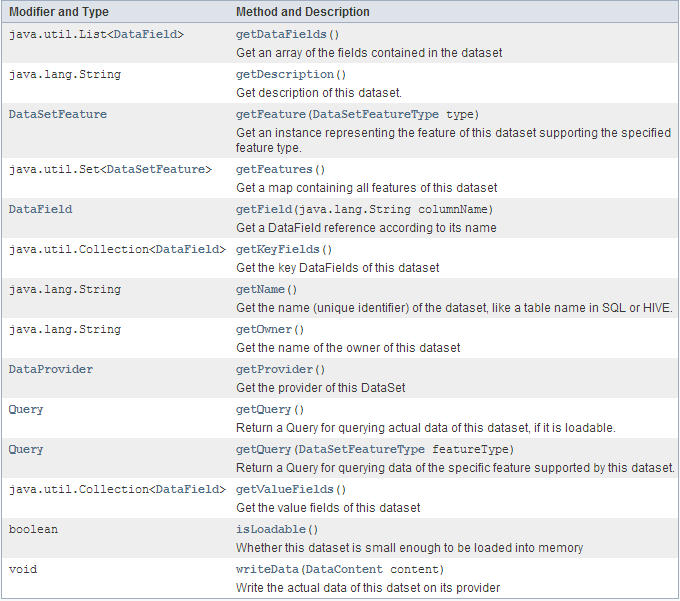
\includegraphics[width=15cm]{dataset.png}
  \label{system:fig:dataset}
\end{table}

数据集的管理通过数据访问对象(Data Access Object,DAO):\texttt{DataSetManager} 来实现。所有数据集的元数据信息以XML形式持久化存储,\texttt{DataSetManager} 封装了数据集新增、查找、更新、保存等多种操作,是获取数据集元数据的唯一途径。

数据列用来描述数据集格式,代表表格型数据中的一列。数据列可能数据某一数据集,也可能在查询中动态生成。数据列的元数据包括数据列名称、类型、语义类型、描述、是否为主键、列值是否有序、以及其所属的数据集等。

\textbf{数据集语义信息管理.} 
为了满足可视化等需要,平台提供了数据集语义信息管理的API。语义信息分为两个层面:数据列语义信息和数据集语义信息。

数据列的语义信息通过记录数据列的语义类型来实现,平台中规定了若干种移动环境下常见的语义类型,见表\ref{system:tab:columnTypes}。根据数据列的语义类型,可将数据列分为两类。一类为属性列,即该列的值代表了观察此数据集的一个维度,可以根据这一列对数据集进行分组统计等进一步分析处理;另一类为实时列,也即值列。这一类的列通常为统计数值或其他数值,可作为进一步统计的目标列,以及用来可视化的数值对象。

\begin{table}
\centering
\caption{数据列的语义类型表}
\label{system:tab:columnTypes}
\begin{tabular}{|c|c|l|} \hline
名称 & 类型 & 描述\\ \hline
纬度 & 属性列 & 地理位置中的纬度\\ \hline
经度 & 属性列 & 地理位置中的经度\\ \hline
编号 & 属性列 & 记录的唯一编号\\ \hline
时间戳 & 属性列 & 记录的时间属性\\ \hline
计数 & 事实列 & 统计数值 \\ \hline
值 & 事实列 & 一般的事实列 \\
\hline\end{tabular}
\end{table}

数据集的语义信息依赖于其包含的所有数据列的语义信息。一个数据集的语义信息主要是其包含哪些属性列的组合。另外,事实列与属性列的搭配关系也属于数据集层面的语义关系。

\textbf{底层数据存储实现的封装.} 

通过规定数据集操作的通用API,屏蔽了底层数据存储实现的细节。在平台中,不同的数据存储实现均作为系统的一个数据提供者(DataProvider)。操作数据集时并不需要关系其后台使用的是哪一个具体的数据提供者。接口 \texttt{DataProvider} 的描述见表\ref{system:fig:dataprovider}。目前已经实现的数据提供者有Hadoop(Hive),JDBC以及纯文本文件。

\begin{table}[htbp]
  \centering 
   \caption{\texttt{DataProvider}接口规范}
    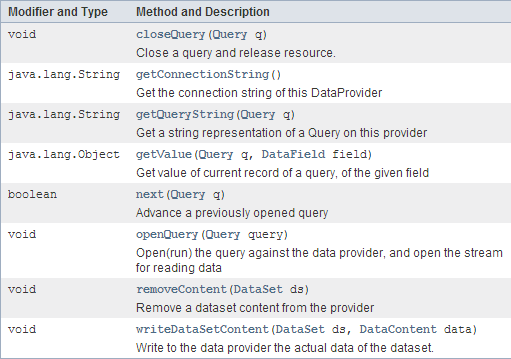
\includegraphics[width=12cm]{provider.png}
  \label{system:fig:dataprovider}
\end{table}

平台提供了数据访问对象 \texttt{DataProviderManager}来对DataProvider进行集中注册和管理。

\textbf{数据查询和访问.} 

为了实现与存储平台的无关性,平台提供了用于查询、遍历和写入数据集数据的通用API。API规定了类 \texttt{DataContent} 作为承载数据内容的对象,通过遍历 \texttt{DataContent}可以得到其每一条记录、每一数据列的值。
获取 \texttt{DataContent}对象,可以通过手动将其他表格型数据转换为 \texttt{DataContent},也可以通过构建 \texttt{Query}对象。\texttt{Query} 类为 \texttt{DataContent}类的子类,负责查询平台上的一个或多个数据集的内容。作为 \texttt{DataContent} 的子类,\texttt{Query} 也可被遍历而得到其数据内容。\texttt{Query} 支持按记录过滤\texttt{where}、按列过滤\texttt{select}、按某些列进行分组统计、排序和内连接等操作。用户可以不关心底层实现,通过调用 \texttt{Query} 对象提供的方法构造各种复杂的查询以满足其需要。各个不同的数据提供者(\texttt{DataProvider})负责将 \texttt{Query} 对象携带的查询信息转换为自身支持的查询格式,并返回查询结果。\texttt{Query} 的描述见表\ref{system:fig:query}

\begin{table}[htbp]
  \centering 
   \caption{\texttt{Query}接口规范}
    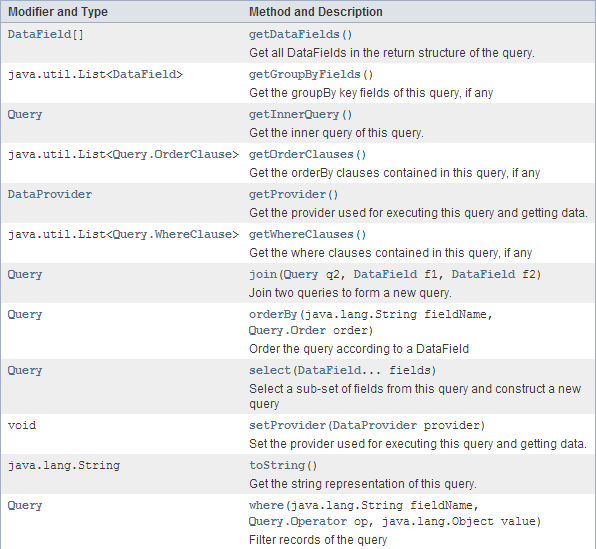
\includegraphics[width=15cm]{query.png}
  \label{system:fig:query}
\end{table}

\subsection{平台远程访问的REST接口设计与实现}
\label{system:sec:restapi}

出于对响应速度、层次的划分的清晰度、扩展度以及开发的便利程度等方面的考虑,平台采用了REST API作为的对外的远程访问接口\cite{pautasso2008restful}。使用REST API,客户端可以利用浏览器的缓存提高用户的响应速度,并且简化了客户端开发和部署的复杂性。

对应与提供后台的数据服务,以及满足平台管理的不同方面的需求,MDAP中的REST API根据功能分为三类:
\begin{itemize}
  \item 数据操作API
  \item 用户管理API
  \item 平台管理API
\end{itemize}

数据操作API对应与平台中队数据集的所有操作,是REST API中最核心的部分。用户可以通过调用数据操作API,设定所需要的参数进行对数据的查询、读取等一系列操作。可以根据数据集的类别、性质、所支持的语义特征等进行针对性的查找。同时针对可视化等前端需求,返回符合要求的多种不同格式的数据集元数据和内容数据。REST API还支持对数据集的增,删,改,查的一系列基本功能,使得使用平台的数据挖掘开发人员和数据分析员可以简单快捷地搭建轻量级的数据探索和展示应用。数据操作API概览见表\ref{system:tab:restapi}。
 
\begin{table}
\centering
\caption{数据操作REST API概览}
\label{system:tab:restapi}
\begin{tabularx}{15cm}{|p{1.3cm}|l|X|} \hline
类别 & URL & 功能 \\ \hline
\multirow{8}{1.3cm}{GET读取} & /mdap/rest/dsg/getdss & 返回所有数据集列表\\ \cline{2-3} 
 & /mdap/rest/dsg/getgeodss & 返回所有包含地理信息数据集列表\\ \cline{2-3}
 & /mdap/rest/dsg/getstadss & 返回所有包含统计信息数据列表\\ \cline{2-3}
 & /mdap/rest/dsg/getds/\textit{datasetname} & 返回数据集\textit{datasetname}的所有信息\\ \cline{2-3}
 & /mdap/rest/dsg/getgeods/\textit{datasetname} & 返回数据集\textit{datasetname}的地理信息\\ \cline{2-3}
 & /mdap/rest/dsg/getstads/\textit{datasetname} & 返回数据集\textit{datasetname}的统计信息\\ \cline{2-3}
 & /mdap/rest/dsg/getstatds/\textit{datasetname} & 返回数据集\textit{datasetname}的时间序列信息\\ \cline{2-3}
 & /mdap/rest/dsg/getdsfds/\textit{datasetname} & 返回数据集\textit{datasetname}的属性信息 \\ \hline
\multirow{3}{1.3cm}{POST创建} & /mdap/rest/dsp/addds/\textit{datasetname} & 添加数据集\textit{datasetname}\\ \cline{2-3}
 & /mdap/rest/dsp/getdsf/\textit{datasetname} & 返回数据集\textit{datasetname}的fieldname列\\ \cline{2-3}
 & /mdap/rest/dsp/getdsres/\textit{datasetname} & 返回数据集\textit{datasetname}的符合fieldname列的值opr特定value值的所有数据 \\ \hline
DELETE删除 & /mdap/rest/dsd/rmds/\textit{datasetname} & 删除数据集\textit{datasetname} \\

\hline\end{tabularx}
\end{table}

用户管理API支持基于用户和角色的访问控制和权限管理。平台提供标准的注册、登陆和基本信息管理的功能,并将用户账户与底层数据平台相联系。同时,为提供基于用户账户的管理和个性化展示,用户管理API还允许每个用户保存、定制自身关注的数据集和可视化结果。

平台管理API在数据管理、用户管理的基础上,提供了更多的平台管理功能。用户可以通过REST API将调用平台SDK的程序包文件验证身份后上传到平台运行,并通过平台管理API查询任务的运行状态。另外,平台上注册的所有数据提供者,支持的语义信息类型等管理数据,也可通过平台管理API查看。

\section{数据可视化模块}
\label{system:sec:vis}

平台利用数据集保存的语义信息,提供了对不同类别的数据集进行有针对性的、可配置的可视化展示。目前,平台支持两大类数据可视化方法:地图可视化和统计数据可视化。含有\emph{维度}、\emph{经度}(参见第\ref{system:sec:javaapi}章)的数据集即可被地图可视化。平台提供灵活的可视化配置,可选择在地图上显示数据集中其他各种不同的附加信息。地图可视化界面样例参见图
\ref{mdap:fig:map}。

\begin{figure}[htbp]
  \centering
    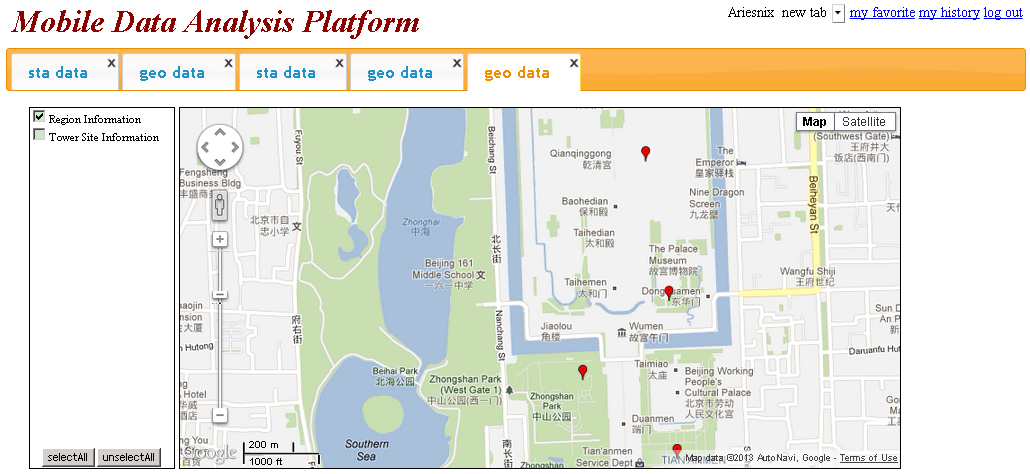
\includegraphics[width=15cm]{geo.png}
  \caption{地图可视化结果样例}
  \label{mdap:fig:map}
\end{figure}
统计可视化则更加灵活。借助数据集的主键域(属性域)和事实域(值域)信息,可灵活使用和配置不同的统计可视化工具,目前支持的有饼图(用以显示比例分布)、折线图(用以显示带时间属性的数据值)、柱状图(对比一个或多个系列的绝对取值大小)等。统计可视化界面样例参见图
\ref{mdap:fig:sta}。


\begin{figure}[htbp]
  \centering
    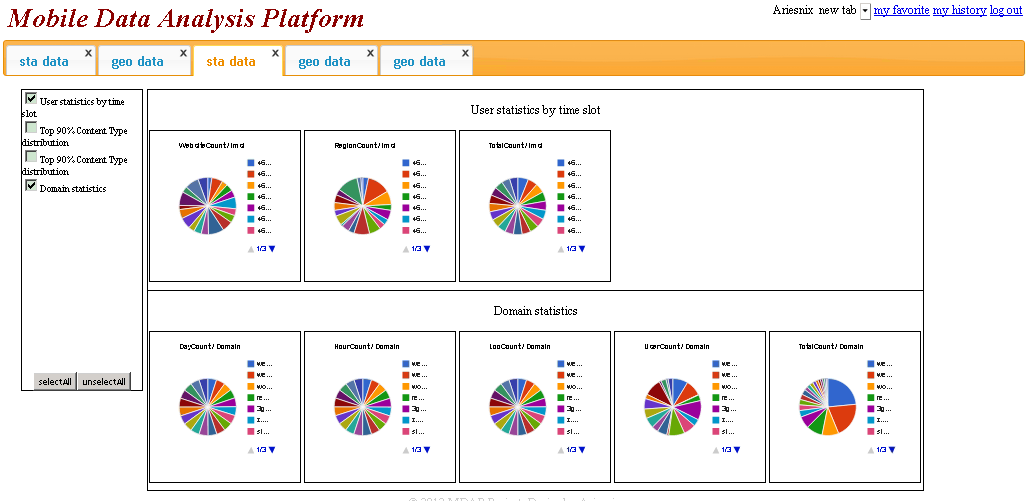
\includegraphics[width=15cm]{sta.png}
  \caption{统计可视化结果样例}
  \label{mdap:fig:sta}
\end{figure}

\section{本章小结}
\label{system:sec:conclusion}

本章展示了用于移动环境下用户行为分析的\textbf{移动用户行为分析平台(Mobile Data Analysis Platform,MDAP)}。首先给出了MDAP的总体架构介绍,包括数据收集模块、数据分析平台和数据展示模块。而后详细描述了Android移动平台上的数据收集应用。包括Android平台传感器介绍,应用收集的数据类型、收集方式,以及传感器数据的收集策略和传感器能耗管理策略等。数据分析平台方面,详细描述了以数据集为主要操作对象的编程接口的设计与实现,通过规定标准的数据操控编程接口实现了对底层数据存储细节的屏蔽,以及不同来源、不同存储方式的数据集的统一操作和继集成,同时还给出了平台REST API的详细描述。最后,描述了系统支持图形化数据浏览和数据可视化的模块,实现了对数据集的通用且有针对性的展示和可视化。